% ================================================================================================================
%  ____        _ _     _                     _   _                                            
% | __ ) _   _(_) | __| | ___ _ __      ___ | |_| |__   ___ _ __     _   _ ___  __ _  __ _  ___ 
% |  _ \| | | | | |/ _` |/ _ \ '__|    / _ \| __| '_ \ / _ \ '__|   | | | / __|/ _` |/ _` |/ _ \
% | |_) | |_| | | | (_| |  __/ |      | (_) | |_| | | |  __/ |      | |_| \__ \ (_| | (_| |  __/
% |____/ \__,_|_|_|\__,_|\___|_|       \___/ \__|_| |_|\___|_|       \__,_|___/\__,_|\__, |\___|
%                                                                                    |___/      
% ================================================================================================================

\section[Применение ``CATIA-GDML geometry builder'' за пределами CBM RICH]{Применение ``CATIA-GDML geometry builder'' за\\ пределами CBM RICH}\label{sec:secBuilderOtherUsage}

% ================================================================================================================
\subsection{CBM ECAL frame}\label{sec:secCbmEcalFrame}

MC-модель рамы электромагнитного калориметра ECAL эксперимента CBM была построена на основе имеющей CAD-модели. Были проработаны две версии рамы, соответствующие двум конфигурациям калориметра --- для SIS100 и SIS300. На~\figref{fig:CbmEcalFrame} представлена MC-модель для SIS300 в системе CbmROOT. В данной модели активно используются инструменты для множественного позиционирования объёмов \textit{Array} и \textit{Replica/Division}.

%\centering

\begin{figure}[H]
\centering
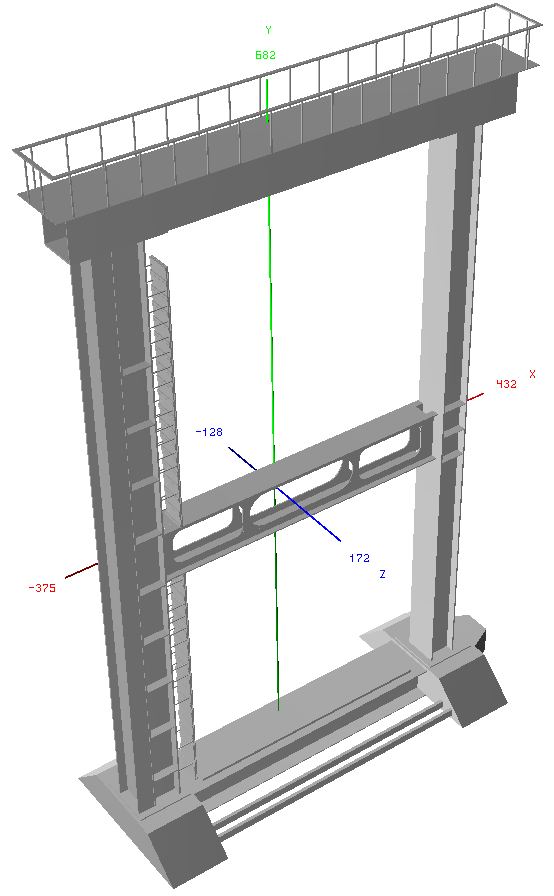
\includegraphics[width=0.4\textwidth]{pictures/CBM_ECAL_frame.png}
\caption{MC-модель рамы электромагнитного калориметра ECAL эксперимента CBM.}
\label{fig:CbmEcalFrame}
\end{figure}

% \begin{figure}[H]
% \begin{minipage}[b]{0.31\textwidth}
% 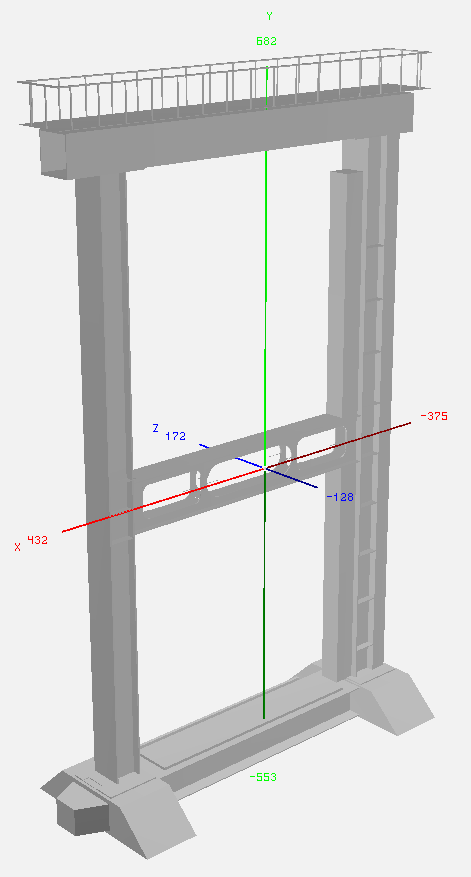
\includegraphics[width=0.95\textwidth]{pictures/ECAL_SIS300_ROOT.png}
% \caption{}
% \label{fig:CbmEcal1}
% \end{minipage}
% \hspace{0.01\textwidth}
% \begin{minipage}[b]{0.31\textwidth}
% 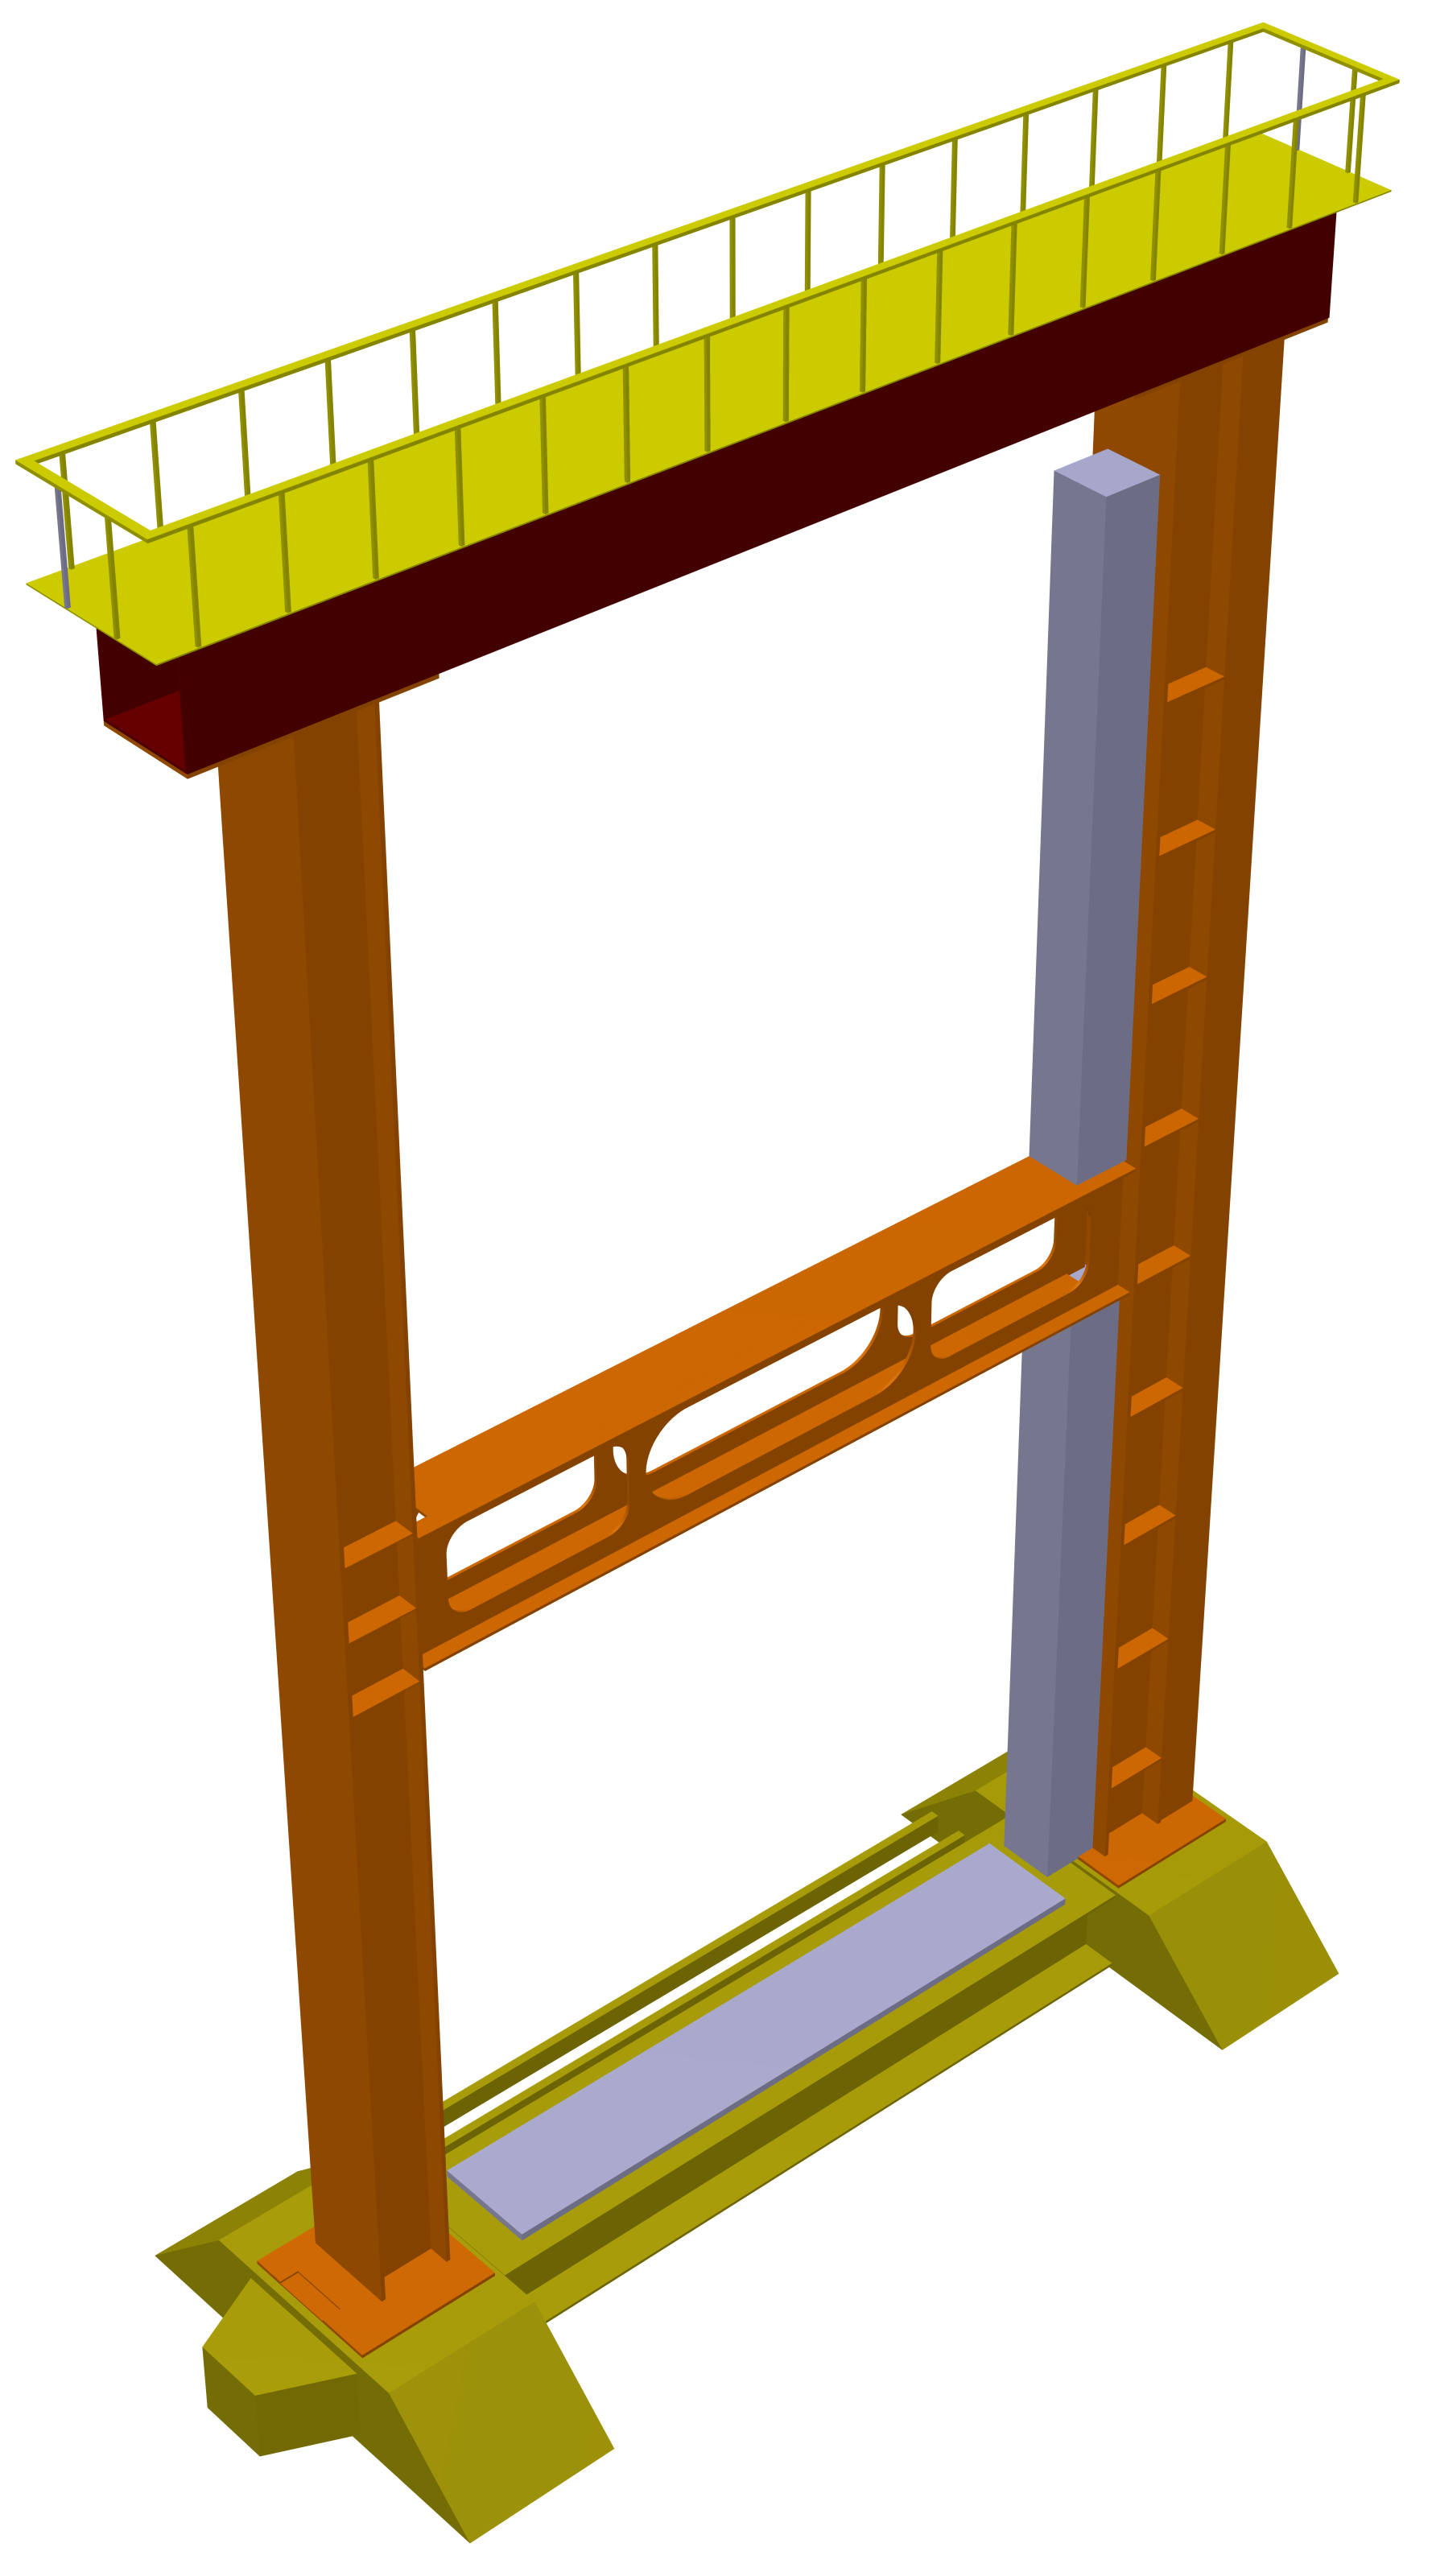
\includegraphics[width=0.95\textwidth]{pictures/ECAL_SIS300_CATIA_g4.png}
% \caption{}
% \label{fig:CbmEcal2}
% \end{minipage}
% \hspace{0.01\textwidth}
% \begin{minipage}[b]{0.31\textwidth}
% 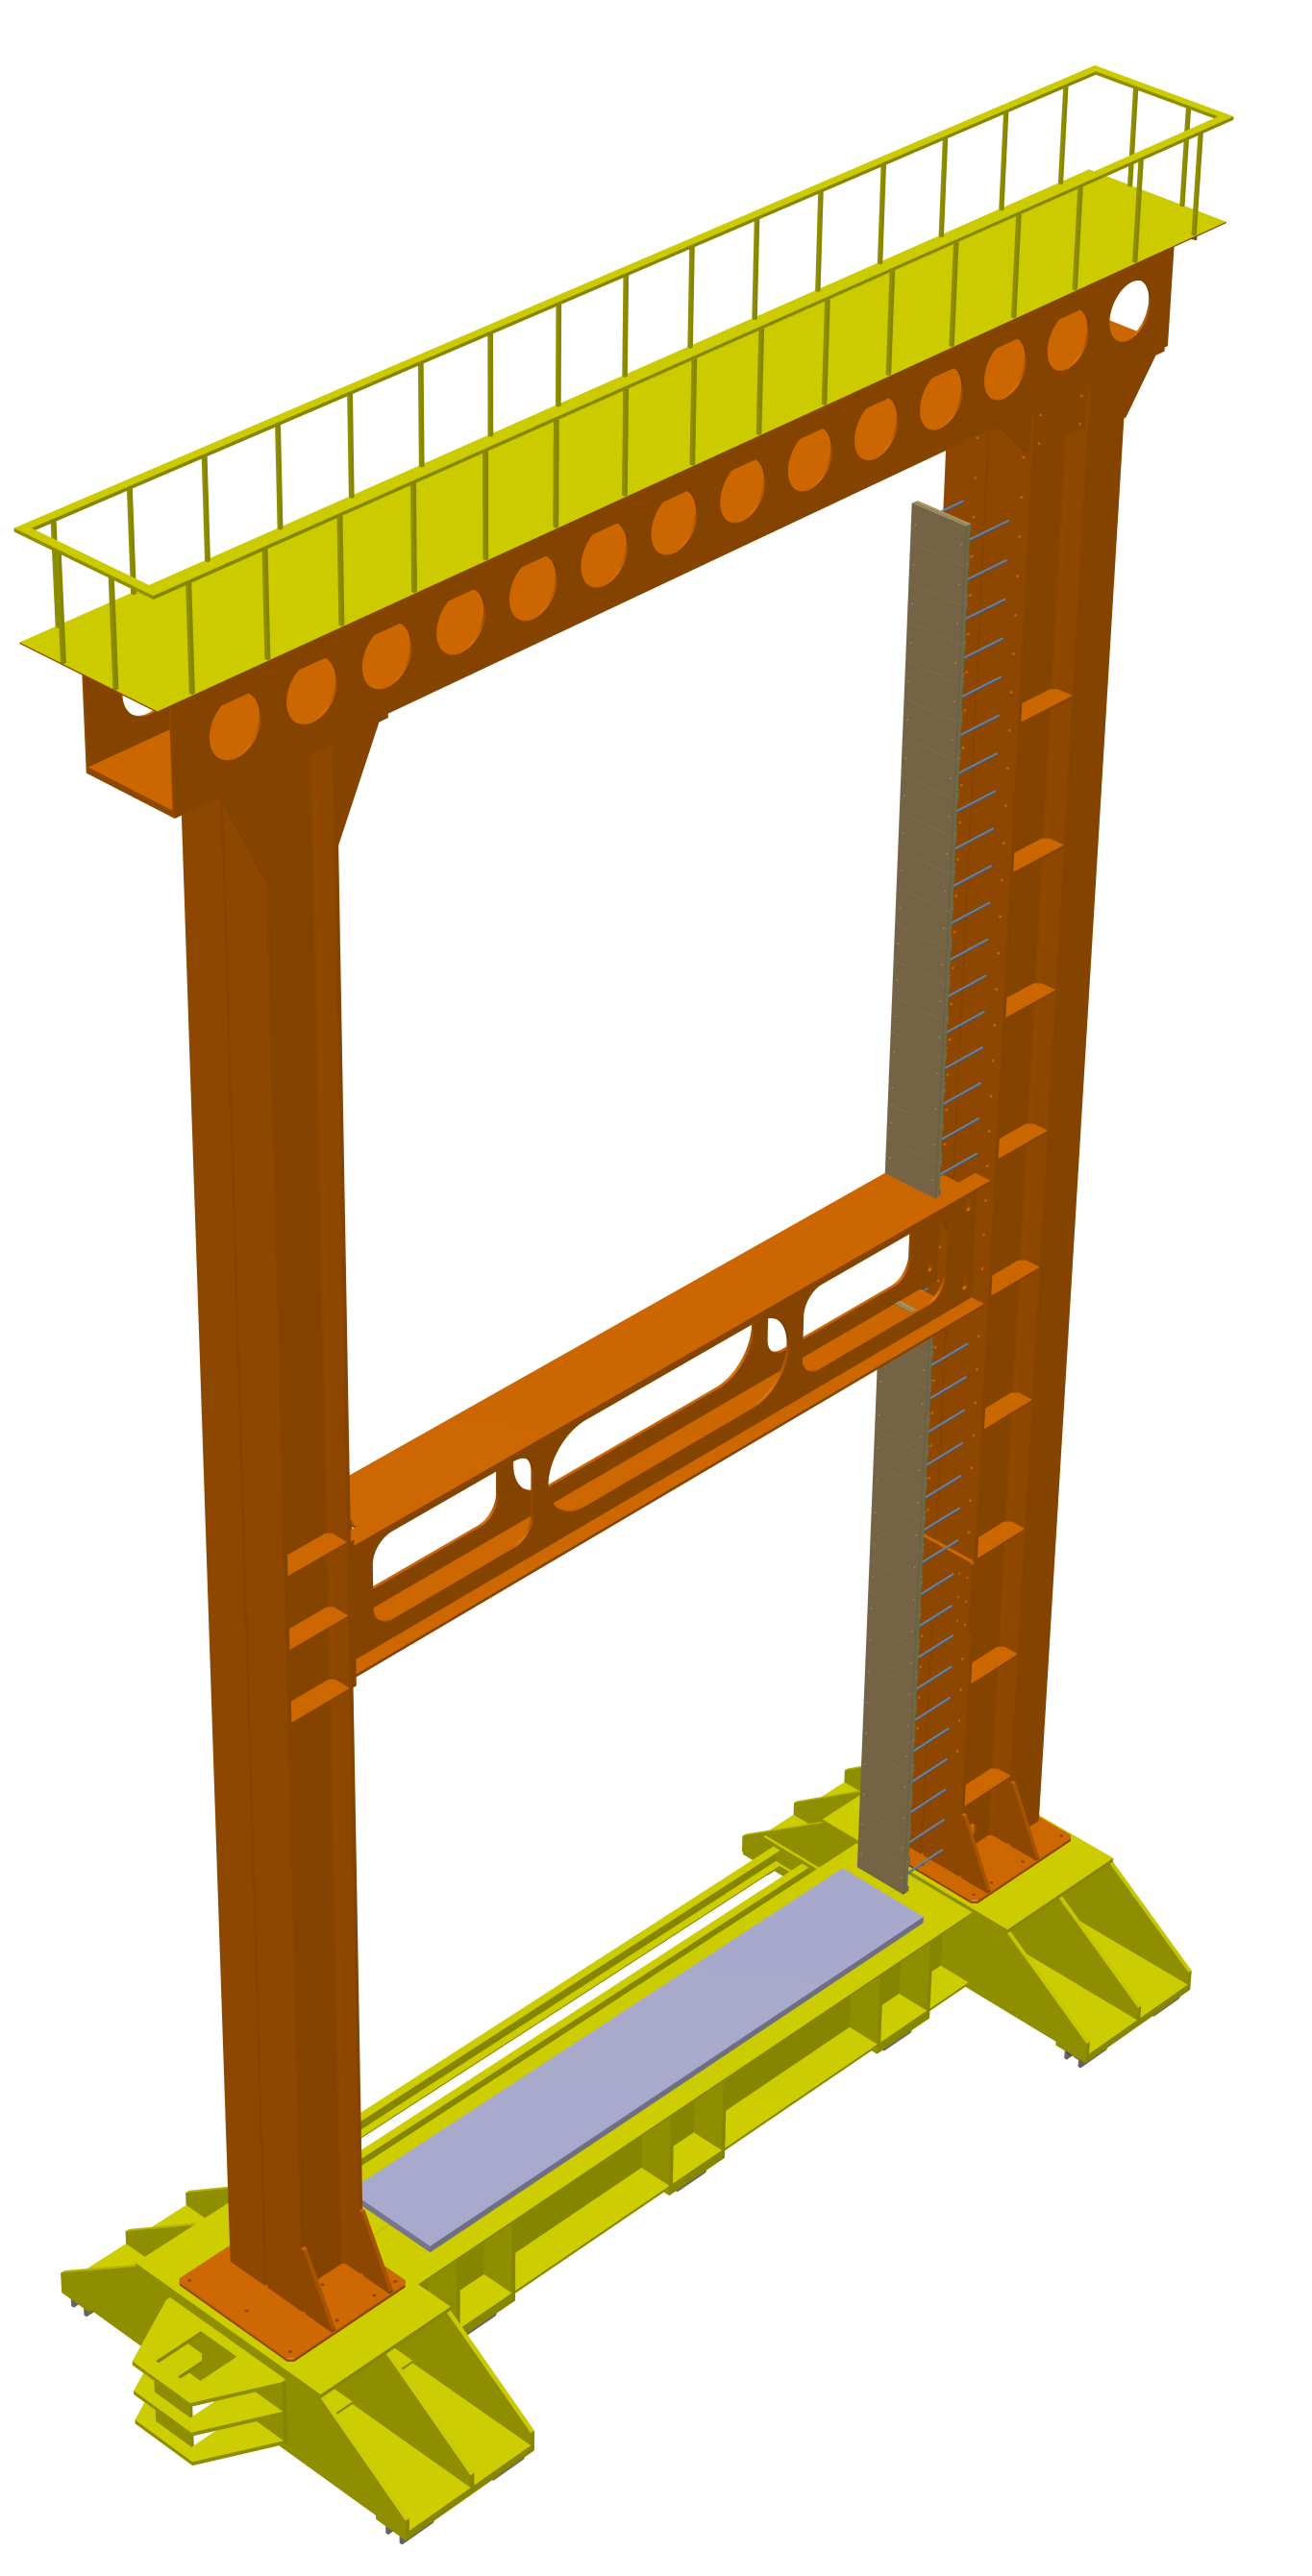
\includegraphics[width=0.95\textwidth]{pictures/ECAL_SIS300_CATIA_cad.png}
% \caption{}
% \label{fig:CbmEcal3}
% \end{minipage}
% \end{figure}

% ================================================================================================================
\subsection{Магнит CBM}\label{sec:secCbmMagnet}

В CBM рассматривалось два совершенно различных проекта дипольного магнита. Каждый из проектов сначала был проработан инженерами и расчётчиками, а затем с помощью ``CATIA-GDML geometry builder'' были последовательно построены обе MC-модели и интегрированы в CbmRoot.
Отличительной особенностью данных MC-моделей является широкое применение разбиения одного твёрдого тела на примитивные составляющие блоки, которые позиционируются рядом на одном уровне, что позволяет избежать применения Булевых операций.
Первая конструкция магнита (см.~\figref{fig:OldCbmMagnet1} и~\figref{fig:OldCbmMagnet2}) была отброшена по причине \todo
Второй проект (см.~\figref{fig:NewCbmMagnet1}) является итоговым и он будет реализован в эксперименте.

\begin{figure}[H]
\begin{minipage}[b]{0.49\textwidth}
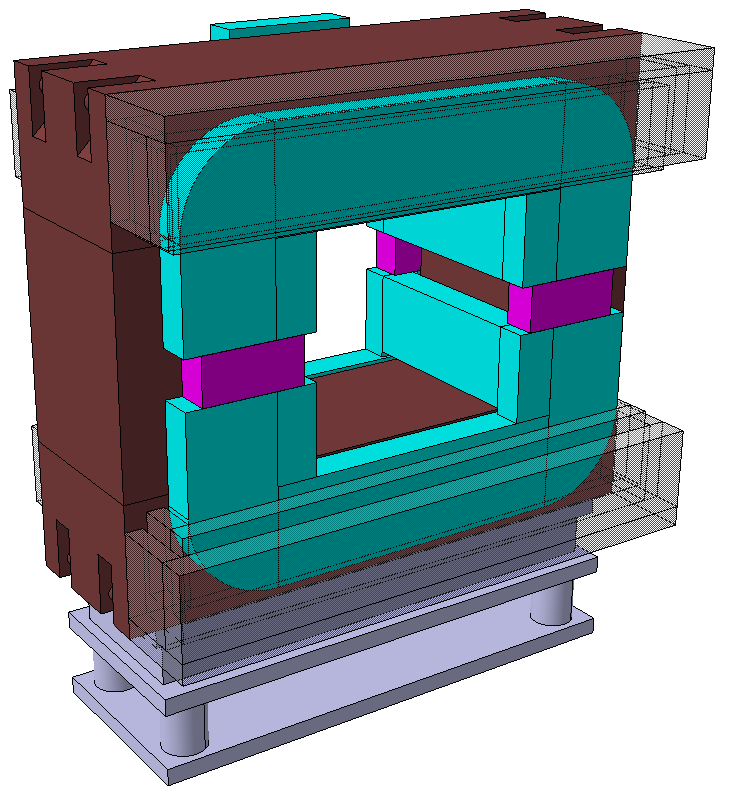
\includegraphics[width=1.0\textwidth]{pictures/Old_magnet_2.png}
\caption{MC-модель прошлой версии дипольного магнита эксперимента CBM.}
\label{fig:OldCbmMagnet1}
\end{minipage}
\hspace{0.01\textwidth}
\begin{minipage}[b]{0.49\textwidth}
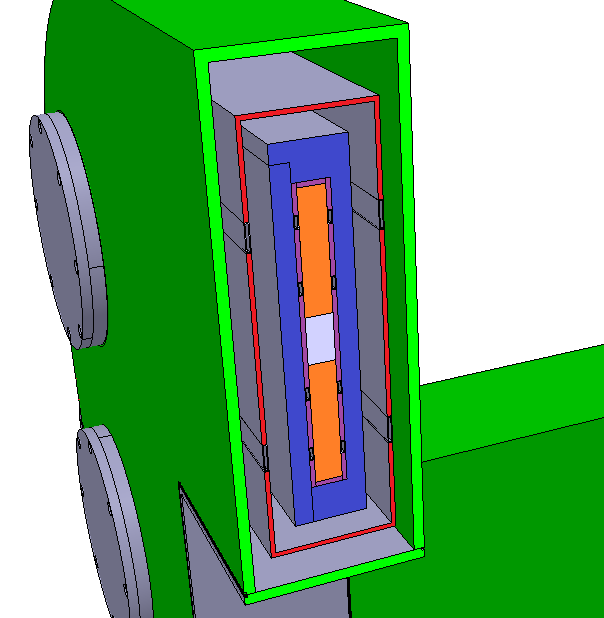
\includegraphics[width=1.0\textwidth]{pictures/Old_magnet_coils.png}
\caption{Внутренняя структура обмоток в MC-модели прошлой версии магнита CBM.}
\label{fig:OldCbmMagnet2}
\end{minipage}
\end{figure}

\begin{figure}[H]
\centering
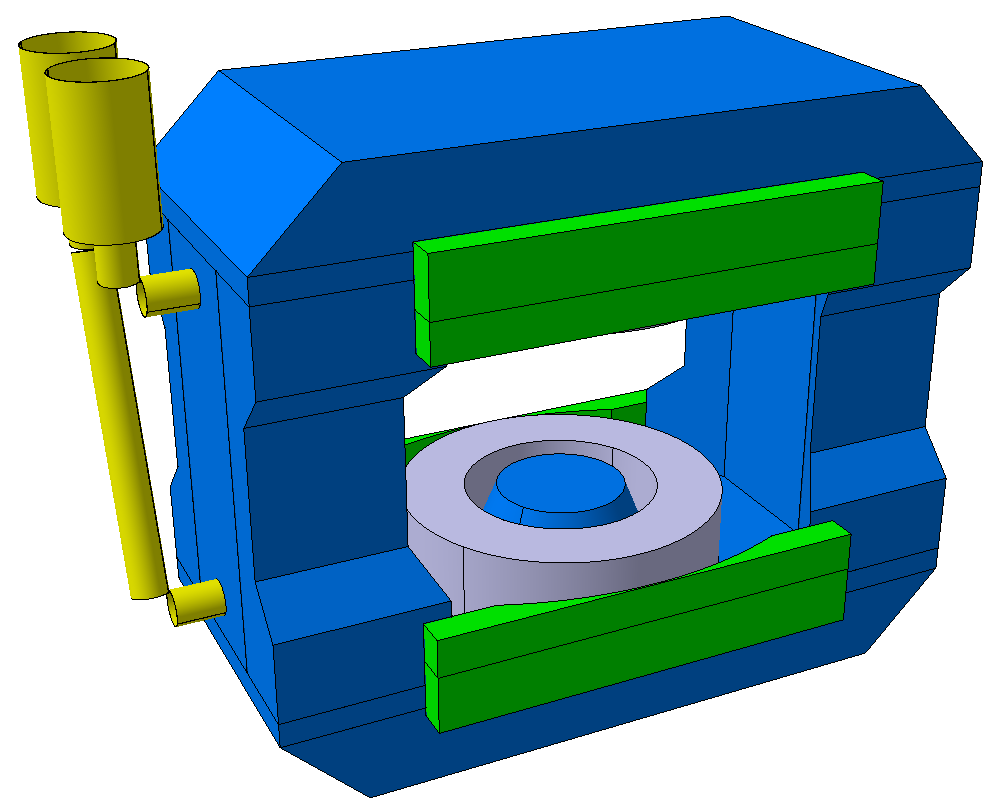
\includegraphics[width=0.7\textwidth]{pictures/New_CBM_magnet.png}
\caption{MC-модель новой версии дипольного магнита эксперимента CBM.}
\label{fig:NewCbmMagnet1}
\end{figure}

% ================================================================================================================
\subsection{R3B GLAD}\label{sec:secGlad}

Помимо эксперимента CBM пакет ``CATIA-GDML geometry builder'' применялся в ряде других проектов, в том числе проектов FAIR. Один из примечательных случаев использования ``Builder'' --- это для построения а основе инженерной CAD-модели корпуса широкоапертурного магнита GLAD (GSI Large Acceptance Dipole) эксперимента R3B (Reactions with Relativistic Radioactive Beams), входящего в группу NUSTAR (Nuclear STructure, Astrophysics and Reactions).

На~\figref{fig:GLAD4} приведена исходная инженерная модель. Корпус имеет сложную внешнюю форму, которую невозможно построить точно с помощью примитивов. Рассматривалось два варианта: аппроксимировать c зазором, но ближе, или без зазора, но дальше \todo доделать

\begin{figure}[H]
\begin{minipage}[b]{0.49\textwidth}
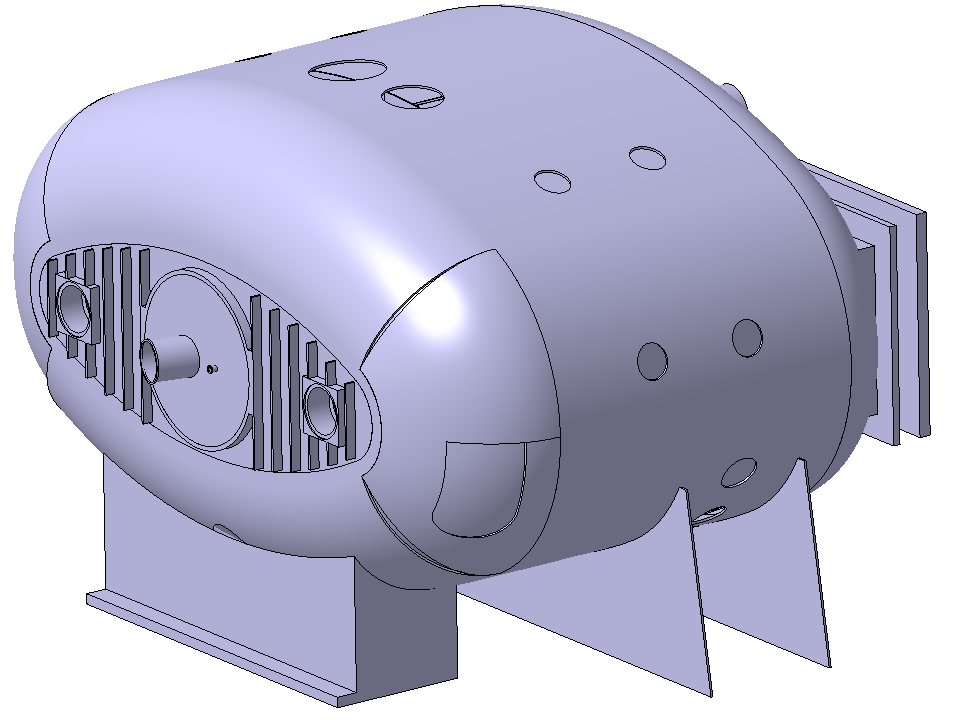
\includegraphics[width=1.0\textwidth]{pictures/GLAD1.png}
\caption{MC-модель.}
\label{fig:GLAD1}
\end{minipage}
\hspace{0.01\textwidth}
\begin{minipage}[b]{0.49\textwidth}
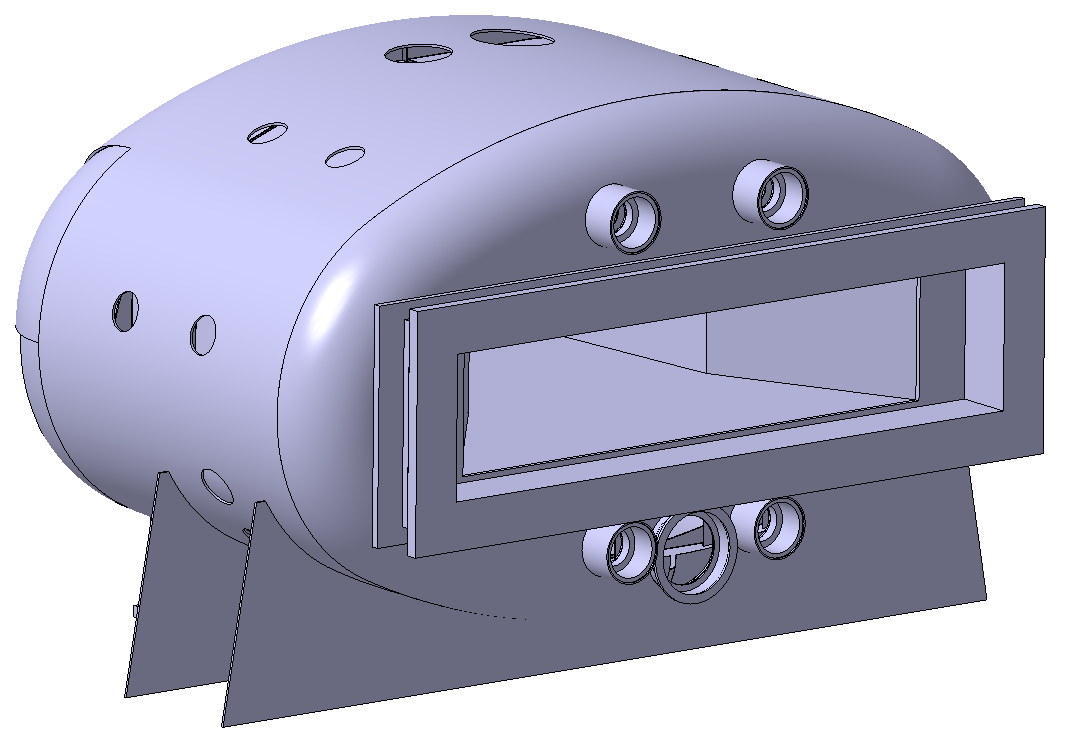
\includegraphics[width=1.0\textwidth]{pictures/GLAD2.png}
\caption{MC-модель.}
\label{fig:GLAD2}
\end{minipage}

\begin{minipage}[b]{0.49\textwidth}
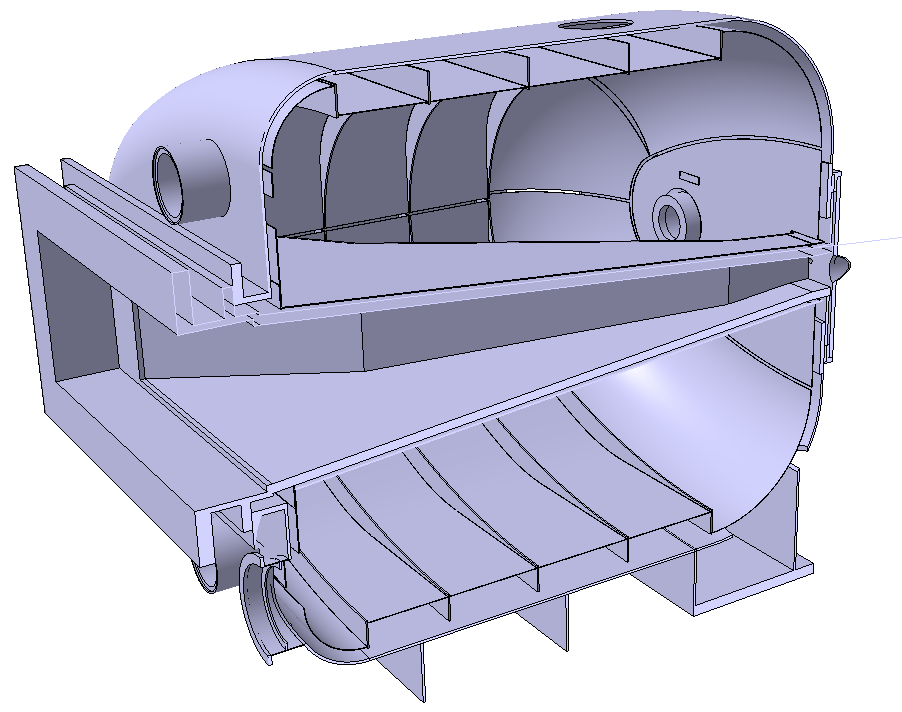
\includegraphics[width=1.0\textwidth]{pictures/GLAD3.png}
\caption{Разрез MC-модели.}
\label{fig:GLAD3}
\end{minipage}
\hspace{0.01\textwidth}
\begin{minipage}[b]{0.49\textwidth}
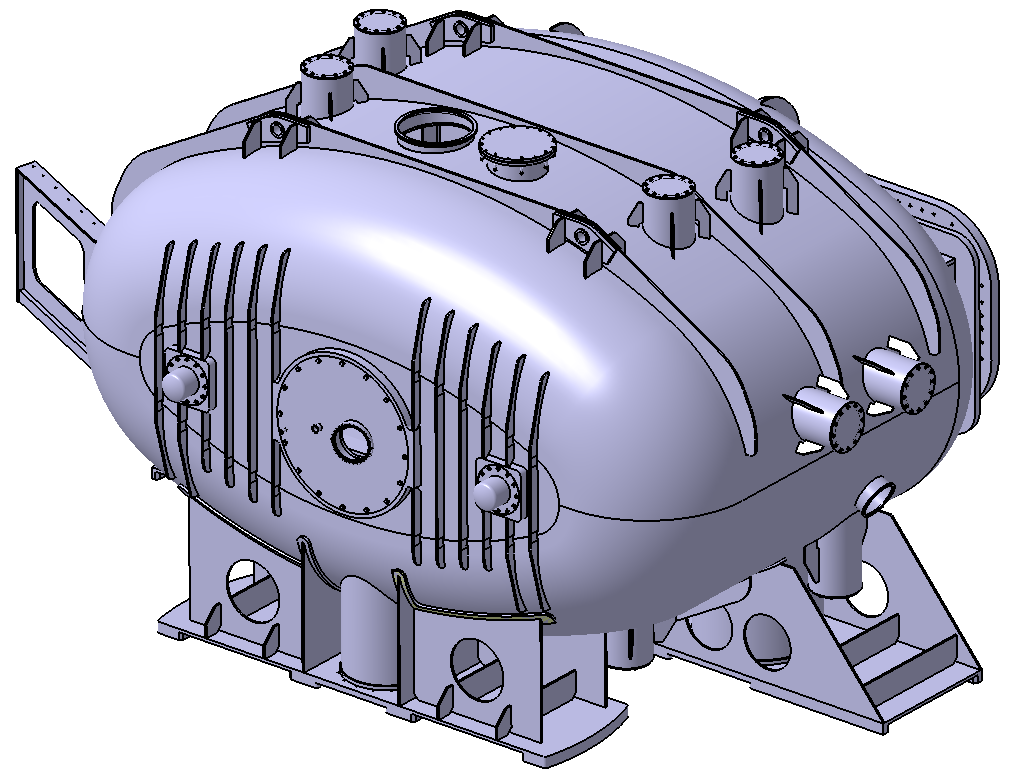
\includegraphics[width=1.0\textwidth]{pictures/R3B_GLAD_CAD.png}
\caption{Исходная инженерная модель.}
\label{fig:GLAD4}
\end{minipage}
\end{figure}

% ================================================================================================================
\subsection{Мюонная система эксперимента CMS}\label{sec:secCmsMuon}

Стояла задача сравнения моделей, заложенных в МК-моделировании, с инженерными моделями, отражающими реальную геометрию изготовленных деталей. Для этого из ROOT был экспортирован GDML файл, который затем был импортирован в CATIA с помощью \macroname{GDML2CATIA}. На~\figref{fig:CmsMuon} показан разрез МК-модели, импортированной в CATIA.

\begin{figure}[H]
\centering
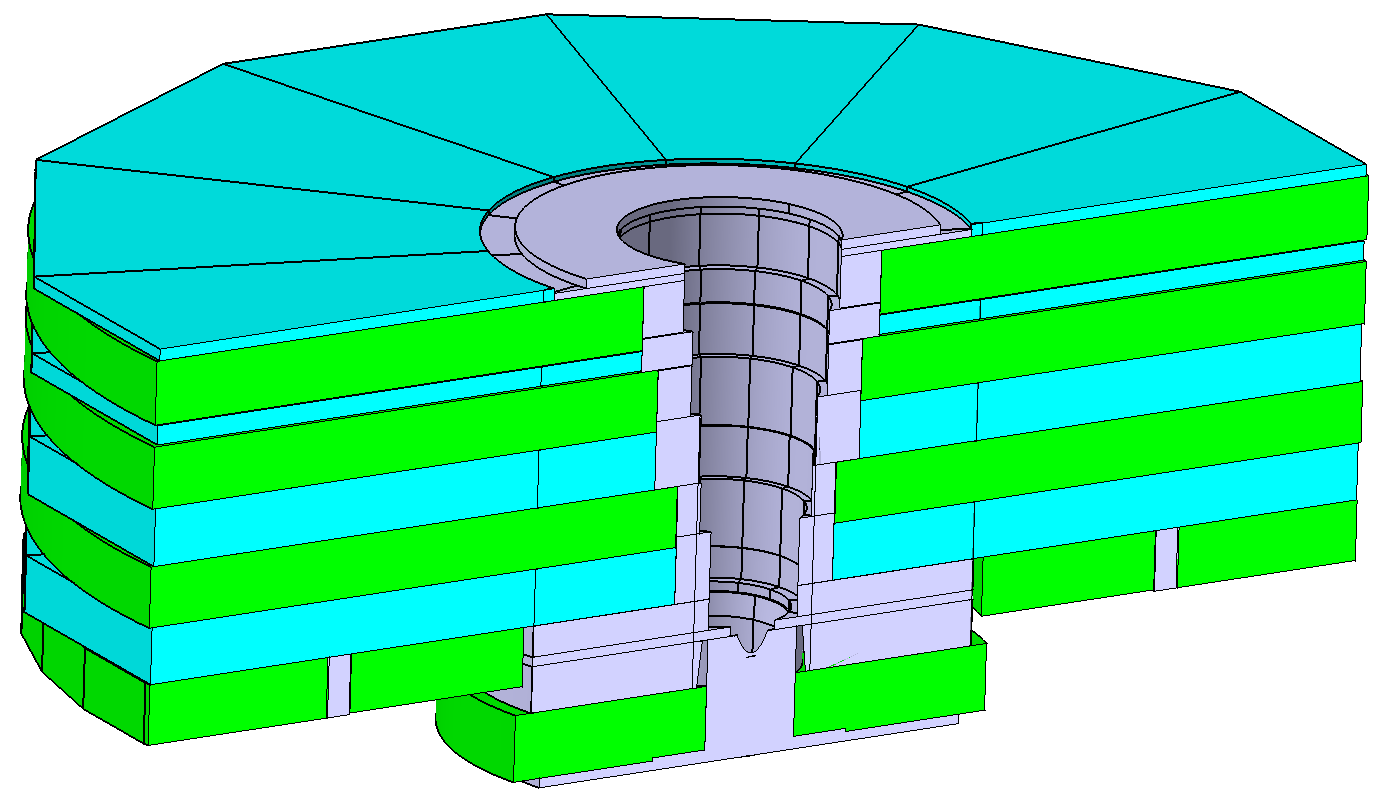
\includegraphics[width=0.7\textwidth]{pictures/CMS_MUON.png}
\caption{Разрез MC-модели мюонной системы эксперимента CMS, импортированной из GDML файла, экспортированного из ROOT.}
\label{fig:CmsMuon}
\end{figure}

% ================================================================================================================
\subsection{Мюонная система эксперимента PANDA}\label{sec:secPandaMuon}

Мюонная система эксперимента PANDA (antiProton ANnihilation in DArmstadt)

Создавался с применением \macroname{Duplicator}.

\begin{figure}[H]
\centering
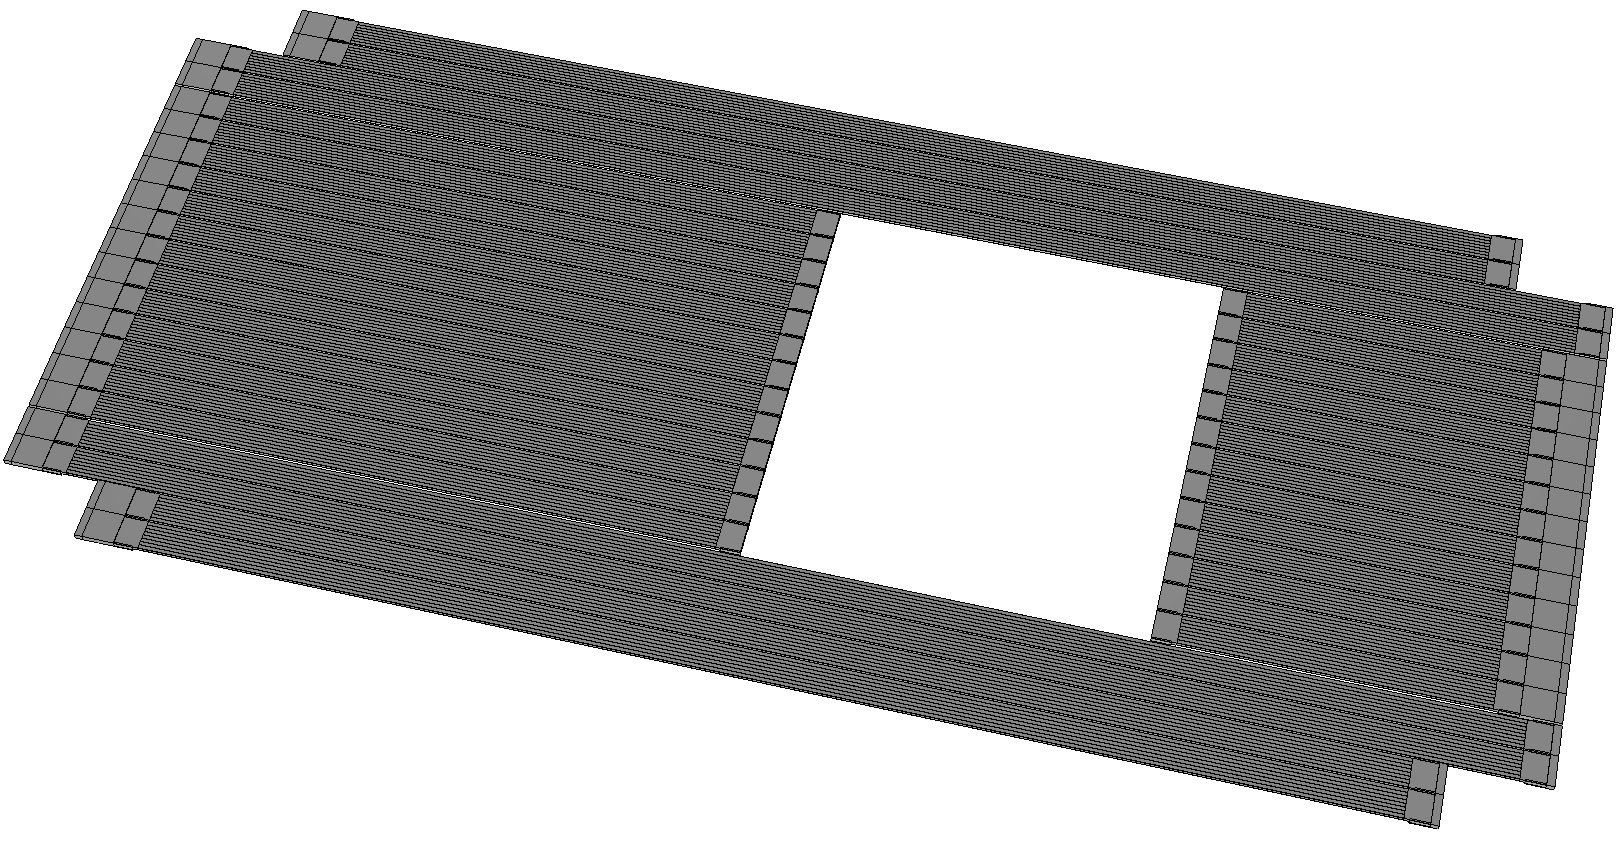
\includegraphics[width=0.7\textwidth]{pictures/PANDA_layer.png}
\caption{MC-модель одного слоя цилиндрической части мюонной системы эксперимента PANDA, созданная в ``CATIA-GDML geometry builder'' с применением \macroname{Duplicator}.}
\label{fig:PandaMuonLayer}
\end{figure}

\begin{figure}[H]
\centering
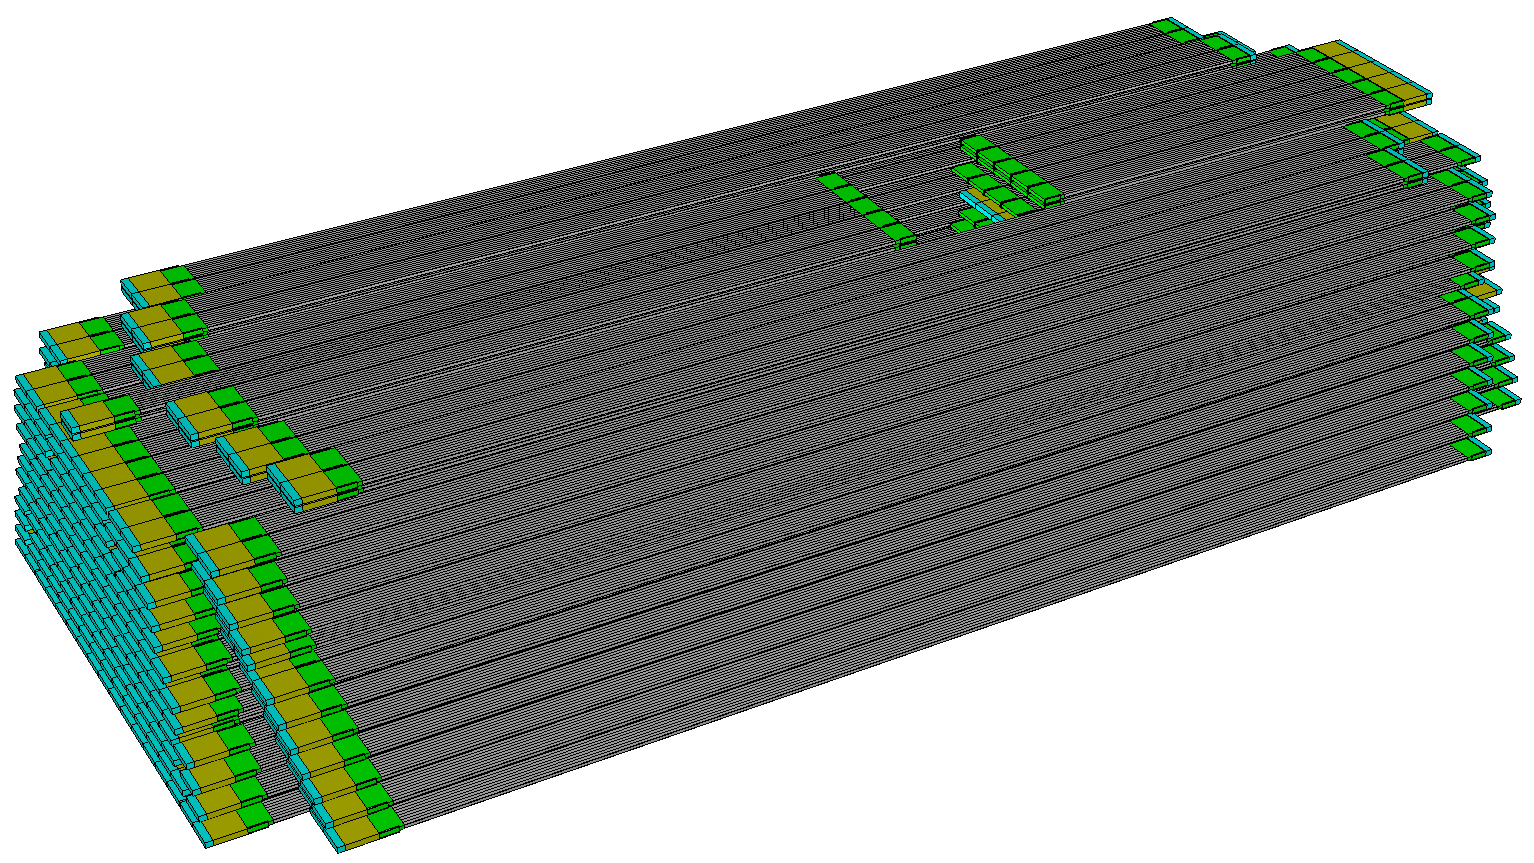
\includegraphics[width=0.7\textwidth]{pictures/PANDA_MUCH_part.png}
\caption{MC-модель сектора цилиндрической части мюонной системы эксперимента PANDA, созданная в ``CATIA-GDML geometry builder''.}
\label{fig:PandaMuonPart}
\end{figure}

% \begin{figure}[H]
% \centering
% 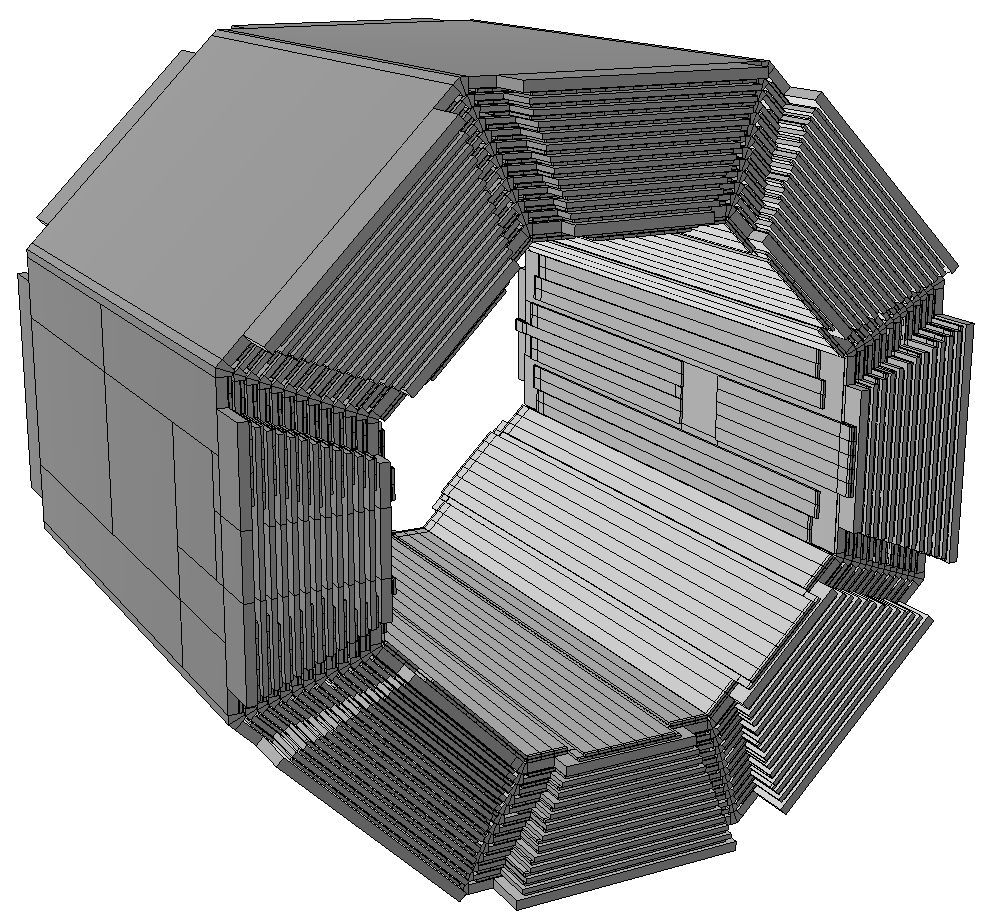
\includegraphics[width=0.7\textwidth]{pictures/PANDA_MUON_barrel.png}
% \caption{}
% \label{fig:PandaMuonBarrel}
% \end{figure}
